\section{Rappresentazione di una mesh}
\label{sec:rappresentazione_mesh}

La maggior parte dei modelli 3D utilizzati in applicazioni reali è composta da complessi di triangoli con vertici condivisi, comunemente detti \emph{mesh triangolari}; gestire questa struttura in modo efficiente è determinante per le prestazioni di un programma grafico, sia in termini di occupazione di memoria su disco che a runtime \cite{marschner2021fcg}. Una mesh triangolare non è un insieme di triangoli tra loro indipendenti, ma una rete di triangoli connessi tramite vertici e archi condivisi a formare un'unica superficie continua: è proprio questa connettività condivisa, e non la semplice somma dei singoli triangoli, a permettere di rappresentare ed elaborare la mesh in modo più efficiente rispetto a una collezione di triangoli scorrelati.

L'informazione minima necessaria per definire una mesh triangolare è l'insieme dei triangoli, ciascuno espresso come tripla di vertici, e la posizione nello spazio di ciascun vertice. La quasi totalità delle applicazioni pratiche, tuttavia, richiede di associare ai vertici (o, a seconda dei casi, agli archi o alle facce) dati aggiuntivi necessari per operazioni come il texture mapping, lo shading o l'animazione. I dati associati ai vertici sono i più comuni: a ciascun vertice possono essere associati parametri di materiale, coordinate texture, o qualunque altra grandezza il cui valore vari con continuità lungo la superficie; tali valori vengono poi interpolati linearmente all'interno di ciascun triangolo, ottenendo così una funzione continua definita sull'intera superficie della mesh.


\subsection{Topologia della mesh}
\label{subsec:mesh_topology}

L'idea che una mesh rappresenti una superficie, e non un insieme arbitrario di triangoli, può essere formalizzata attraverso vincoli sulla sua topologia, ovvero sul modo in cui i triangoli sono connessi tra loro, indipendentemente dalla posizione dei vertici. Il vincolo più semplice e più restrittivo è che la mesh sia una varietà (\emph{manifold}): una mesh manifold non presenta buchi o giunzioni ambigue, e separa in modo netto lo spazio interno alla superficie da quello esterno \cite{marschner2021fcg}. Questa proprietà è alla base del funzionamento di molti algoritmi di elaborazione geometrica, tra cui la struttura dati Half-Edge discussa nella Sezione \ref{subsec:strutture_dati_per_la_connettivita}, che assume implicitamente che la mesh su cui opera sia manifold.

In molte applicazioni è inoltre necessario poter distinguere il lato "esterno" di una superficie da quello "interno", proprietà nota come orientazione. Per un singolo triangolo, l'orientazione è convenzionalmente definita in base all'ordine con cui i suoi vertici sono elencati: il lato anteriore del triangolo è quello da cui i tre vertici appaiono disposti in senso antiorario.


\subsection{Indexed Mesh}
\label{subsec:indexed_mesh_storage}

I triangoli di una mesh possono essere memorizzati come entità indipendenti, ciascuna con i propri tre vertici: questo approccio, tuttavia, comporta la duplicazione dei vertici condivisi da più triangoli, con un evidente spreco di spazio. In alternativa, è possibile memorizzare una sola volta ciascun vertice distinto e far sì che ogni triangolo vi faccia riferimento tramite un indice: questa soluzione, nota come \emph{indexed triangle mesh} (o \emph{shared-vertex mesh}), evita la duplicazione dei dati di vertice ed è la forma di memorizzazione più diffusa nelle applicazioni pratiche.
\begin{figure}[htbp]
	\centering
	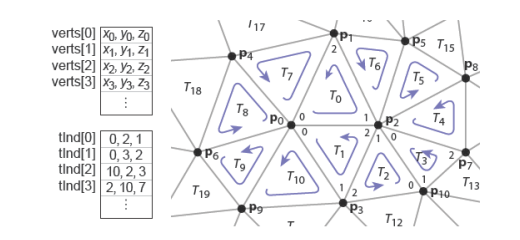
\includegraphics[width=0.75\textwidth]{figures/2_background_teorico/indexed-triangle-mesh.png}
\end{figure}

\subsection{Grafi planari e Planar Straight-Line Graph}
\label{subsec:grafi_planari}

Le strutture dati per la connettività discusse nel seguito derivano concettualmente dall'idea di rappresentare una mesh come un grafo: un insieme di vertici e di archi, a cui si aggiunge un insieme di facce definite come cicli ordinati di vertici o archi. Un grafo è detto planare se può essere disegnato su un piano senza che i suoi archi si intersechino al di fuori dei vertici condivisi; è detto planare embedded (o piano) quando tale disposizione è stata effettivamente fissata nello spazio. Quando, in aggiunta, gli archi sono segmenti rettilinei anziché curve generiche, si parla di \textbf{Planar Straight-Line Graph} (PSLG): è la rappresentazione naturale per dati geometrici 2D costituiti da spezzate e poligoni, ed è tipicamente il punto di partenza per operazioni come l'estrazione delle facce racchiuse dal grafo o la sua triangolazione.
\begin{figure}[htbp]
	\centering
	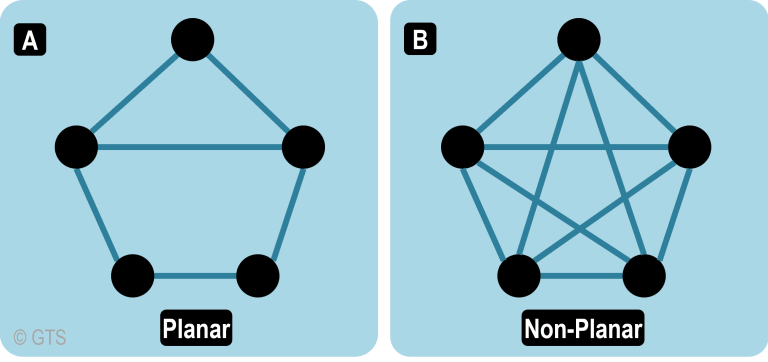
\includegraphics[width=0.5\textwidth]{figures/2_background_teorico/planar_non_planar_graphs.png}
\end{figure}

\newpage

\subsection{Strutture dati per la connettività}
\label{subsec:strutture_dati_per_la_connettivita}

Oltre alla semplice memorizzazione indicizzata, esistono diverse strutture dati pensate per rendere esplicita ed efficiente la navigazione della connettività di una mesh, tanto più rilevanti quanto più le mesh coinvolte sono di grandi dimensioni \cite{marschner2021fcg}.

Una prima soluzione, relativamente semplice, è la \textbf{Triangle-Neighbor Structure}: a partire da una mesh a vertici condivisi, si arricchisce ciascun triangolo con un riferimento ai tre triangoli adiacenti (uno per ciascun lato), e ciascun vertice con un riferimento a uno qualsiasi dei triangoli incidenti su di esso.
\begin{figure}[htbp]
	\centering
	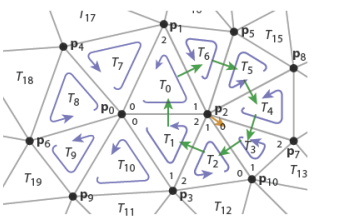
\includegraphics[width=0.5\textwidth]{figures/2_background_teorico/triangle-neighbor-structure.png}
\end{figure}

Una struttura più flessibile, ampiamente utilizzata, è la \textbf{Winged-Edge}, che memorizza l'informazione di connettività a livello di arco anziché di faccia \cite{marschner2021fcg}. In una mesh Winged-Edge, ogni arco memorizza un riferimento ai due vertici che collega (tipicamente indicati come vertice di testa e di coda), alle due facce di cui è parte (la faccia a sinistra e quella a destra), e, soprattutto, agli archi successivo e precedente nella percorrenza in senso antiorario di ciascuna delle due facce adiacenti. Ogni vertice e ogni faccia memorizza inoltre un riferimento a uno qualsiasi degli archi a esso incidenti. Il nome della struttura deriva dal fatto che l'insieme di questi riferimenti, disposti attorno a un singolo arco, assume graficamente la forma di una farfalla con quattro "ali".
\begin{figure}[htbp]
	\centering
	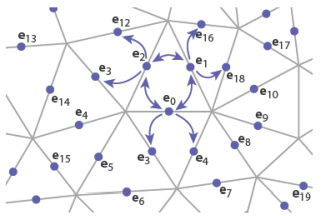
\includegraphics[width=0.5\textwidth]{figures/2_background_teorico/winged-edge-structure.png}
\end{figure}

La struttura Winged-Edge è elegante ma presenta un inconveniente pratico: per spostarsi da un arco al successivo è necessario verificare costantemente da quale lato lo si sta percorrendo, poiché un arco è condiviso da due facce e la sua orientazione dipende dal punto di vista. La struttura \textbf{Half-Edge} (o \emph{doubly-linked edge list}) risolve questo problema suddividendo ciascun arco in due \emph{half-edge} orientati in direzioni opposte, uno per ciascuna delle due facce che condividono l'arco: l'informazione normalmente memorizzata su un singolo arco Winged-Edge viene così distribuita tra i due half-edge, ciascuno coerente con l'orientazione della propria faccia. Ogni half-edge memorizza un riferimento alla faccia sul proprio lato dell'arco, al vertice verso cui punta, al proprio gemello (\emph{twin}, l'half-edge opposto che rappresenta lo stesso arco fisico visto dall'altro lato) e all'half-edge successivo lungo il perimetro della propria faccia. Percorrendo ripetutamente questi riferimenti "successivi" si ottiene un ciclo chiuso corrispondente esattamente al contorno di una faccia, mentre alternando i riferimenti al gemello e al successivo è possibile iterare sugli archi che si dipartono da un dato vertice: proprietà che rende la struttura Half-Edge particolarmente indicata per algoritmi che devono navigare ripetutamente la topologia della mesh, come l'estrazione o la classificazione delle facce racchiuse da un PSLG.
\begin{figure}[htbp]
	\centering
	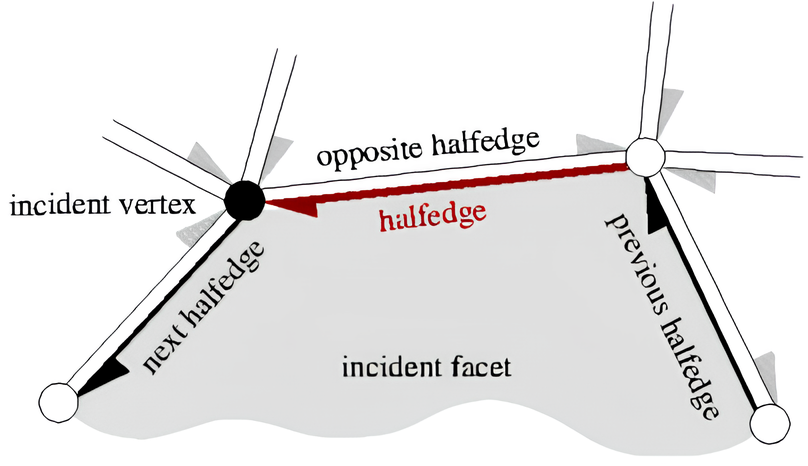
\includegraphics[width=0.5\textwidth]{figures/2_background_teorico/cgal-halfedge.png}
\end{figure}


\subsection{Attributi dei vertici}
\label{subsec:attributi_dei_vertici}

Come discusso in apertura di questa sezione, un vertice può essere arricchito con attributi opzionali oltre alla propria posizione nello spazio; tra questi, due sono di particolare rilevanza per una pipeline di rendering: il vettore normale e le coordinate texture.

Il vettore \textbf{normale} è un vettore unitario perpendicolare alla superficie nel punto considerato, ed è l'informazione che un motore di rendering utilizza per determinare l'orientazione della superficie rispetto a una sorgente luminosa ai fini del calcolo dello shading.

Le \textbf{coordinate texture} associano invece a ciascun vertice una posizione $(u, v)$, con $u, v \in [0, 1]$, all'interno di un'immagine bidimensionale (la texture) usata per aggiungere dettaglio visivo alla superficie senza dover infittire la geometria della mesh. Per applicare correttamente una texture a un triangolo è necessario specificare, per ciascuno dei suoi tre vertici, quale punto della texture gli corrisponde; il resto della superficie del triangolo viene poi campionato per interpolazione tra questi tre valori. Per convenzione, la coordinata $(0,0)$ corrisponde all'angolo inferiore sinistro dell'immagine e $(1,1)$ all'angolo superiore destro. Qualora vengano specificate coordinate al di fuori dell'intervallo $[0,1]$, il comportamento del campionamento dipende dalla modalità di \emph{wrapping} scelta (ripetizione, ripetizione speculare, o clamping ai bordi), un dettaglio implementativo che esula dagli scopi di questa trattazione teorica.